即使在具有移动语义的类型成员(如字符串成员或容器)的类中,也可以受益于移动语义。\par

让我们看一个简单的例子。\par

\hspace*{\fill} \par %插入空行
\textbf{4.3.1 用经典方法初始化成员}

考虑一个有两个string成员的类,我们可以在构造函数中初始化。这样的类通常会这样实现:\par

{\color{red}{basics/customer.hpp}}

\begin{lstlisting}[caption={}]
#include <string>
class Person {
private:
	std::string first; // first name
	std::string last; // last name
public:
	Person(const std::string& f, const std::string& l)
	: first{f}, last{l} {
	}
	...
};
\end{lstlisting}

让我们看看当用两个字符串字面值初始化该类的对象时,会发生什么:\par

\begin{lstlisting}[caption={}]
Person p{"Ben", "Cook"};
\end{lstlisting}

编译器发现提供的构造函数可以执行初始化。但参数的类型不适合。因此,编译器生成代码首先创建两个临时std::string,它们由两个字符串字面量的值初始化,并将形参f和l绑定到它们:\par

\begin{center}
	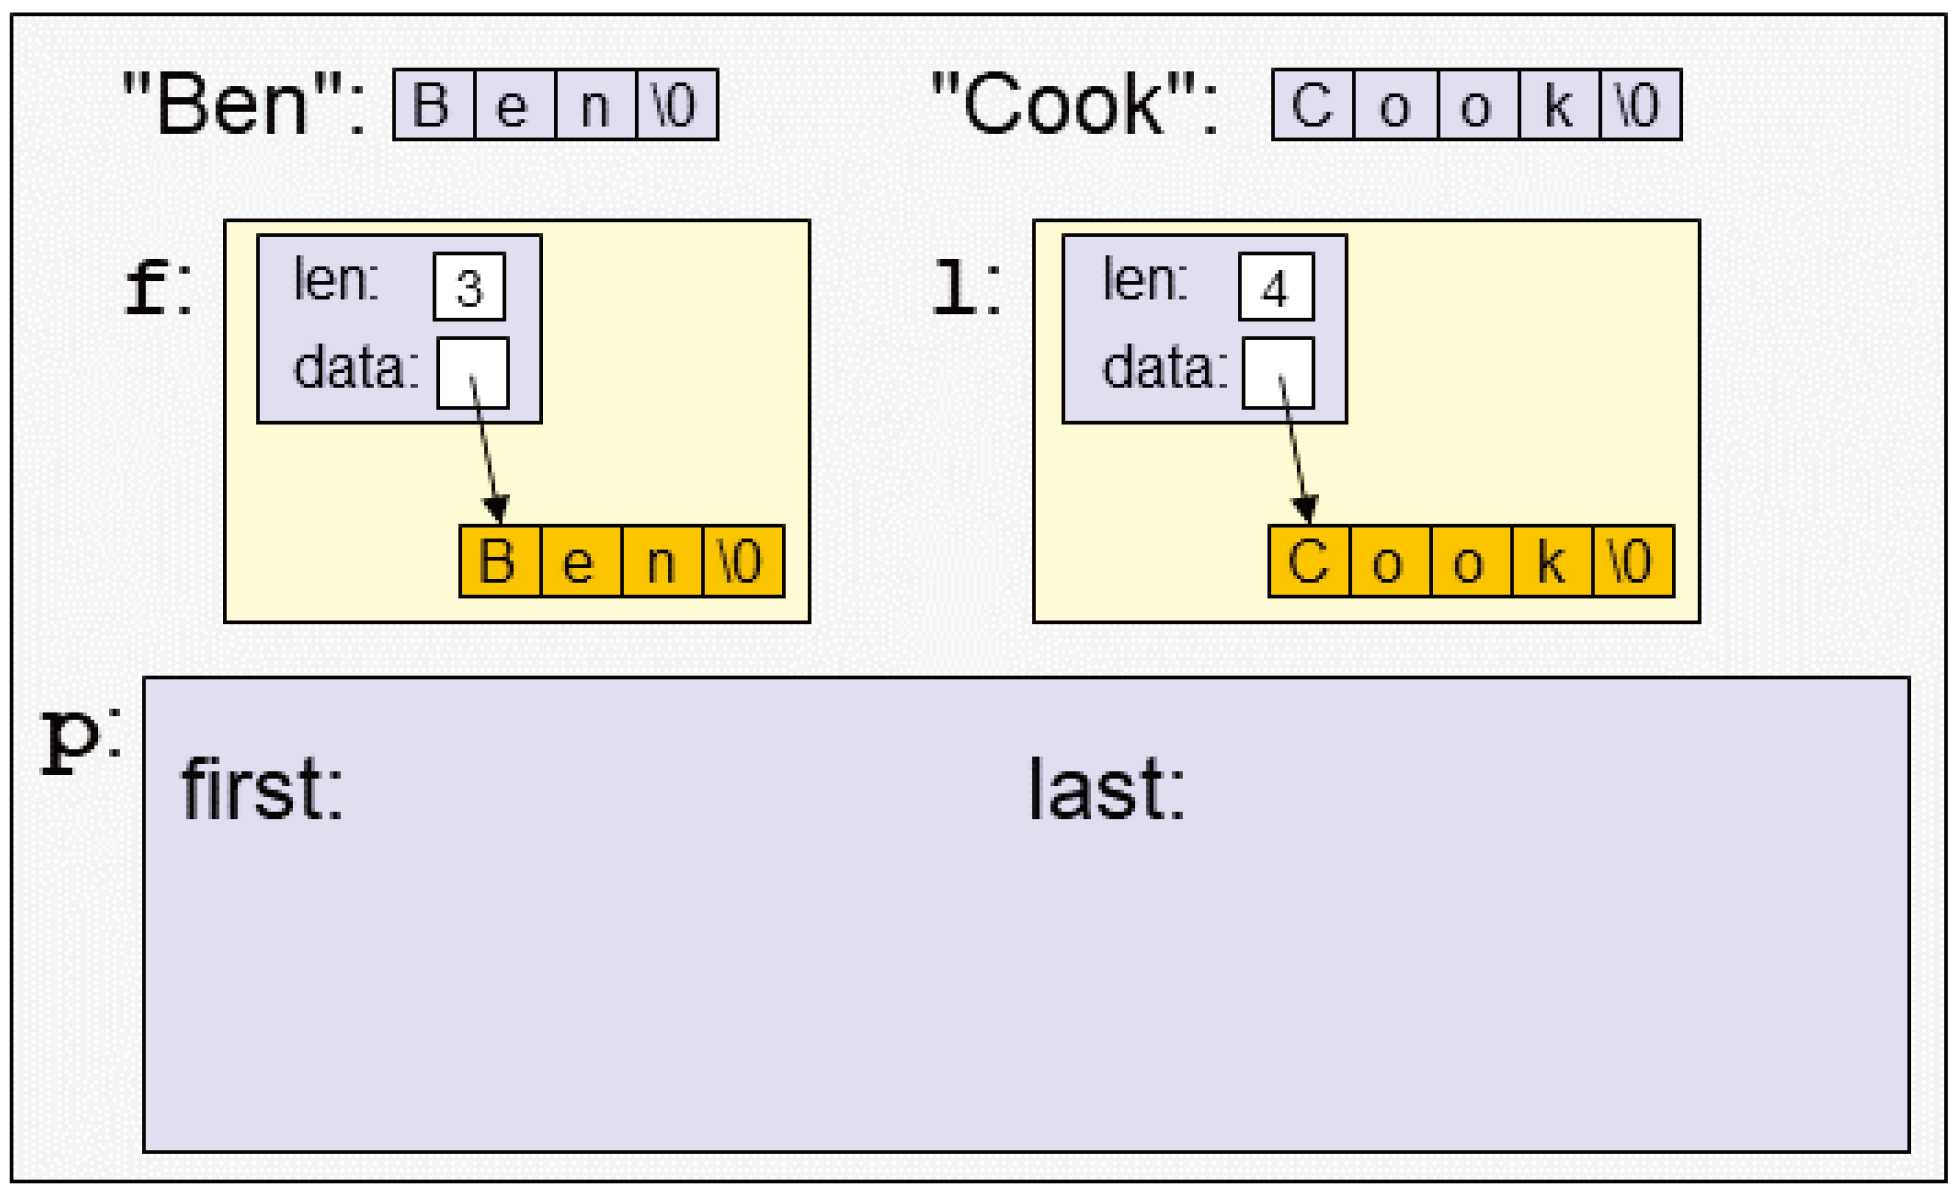
\includegraphics[width=0.6\textwidth]{content/1/chapter4/images/1}
\end{center}

一般来说(如果小字符串优化(SSO)不可用或者字符串太长),这会为每个std::string的值分配内存。\par

创建的临时字符串不能直接作为first或last成员使用,但现在却用于初始化这些成员。不幸的是,这里没有使用移动语义,原因有二:\par

\begin{itemize}
	\item 形参f和l是对象,其名称存在的时间长于成员初始化的时间(仍然可以在构造函数体中使用它们)。
	\item 形参声明为const,即使使用std::move()也禁用move语义。
\end{itemize}

因此,在每个成员初始化时调用string的复制构造函数,会再次为这些值分配内存:\par

\begin{center}
	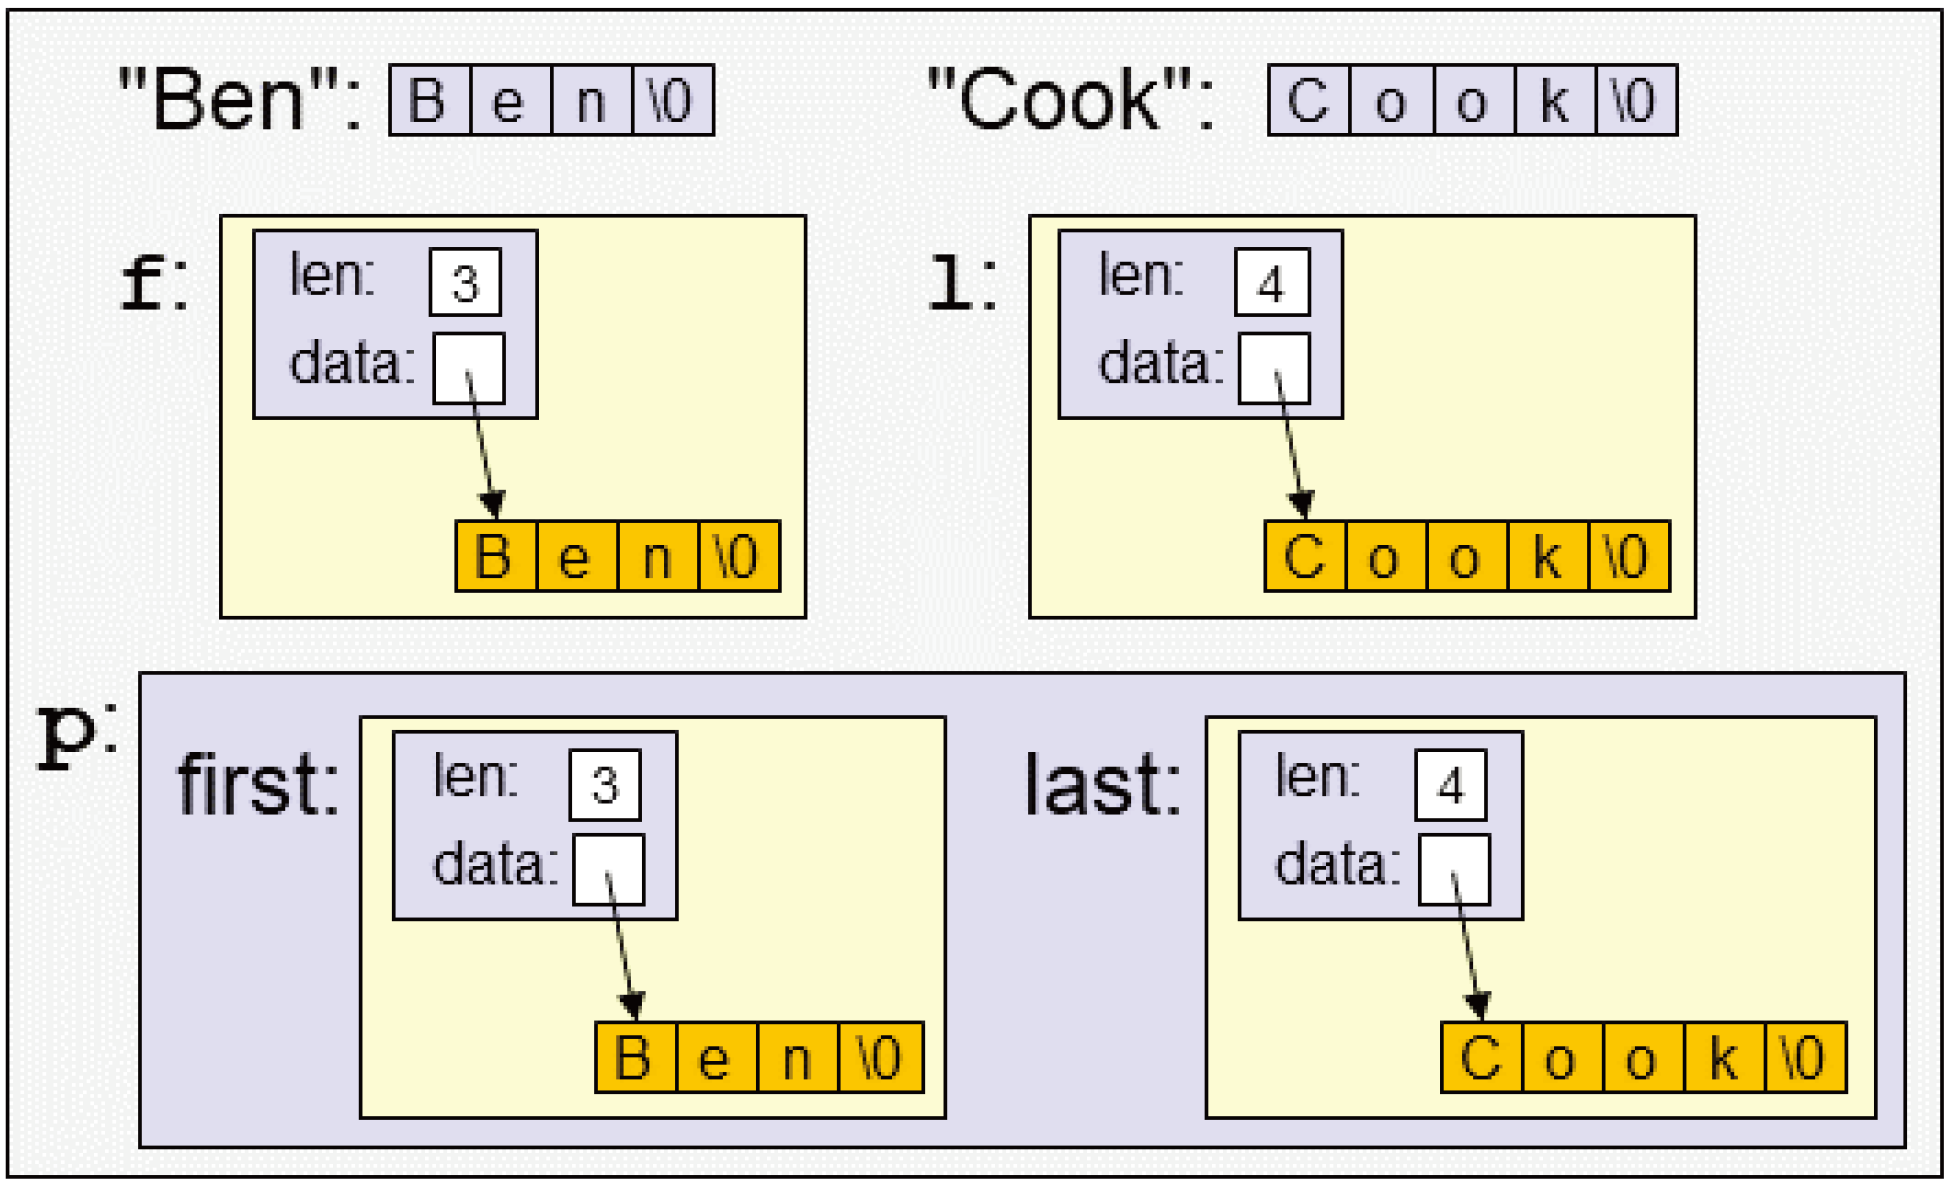
\includegraphics[width=0.6\textwidth]{content/1/chapter4/images/2}
\end{center}

在构造函数的末尾,销毁临时字符串:\par

\begin{center}
	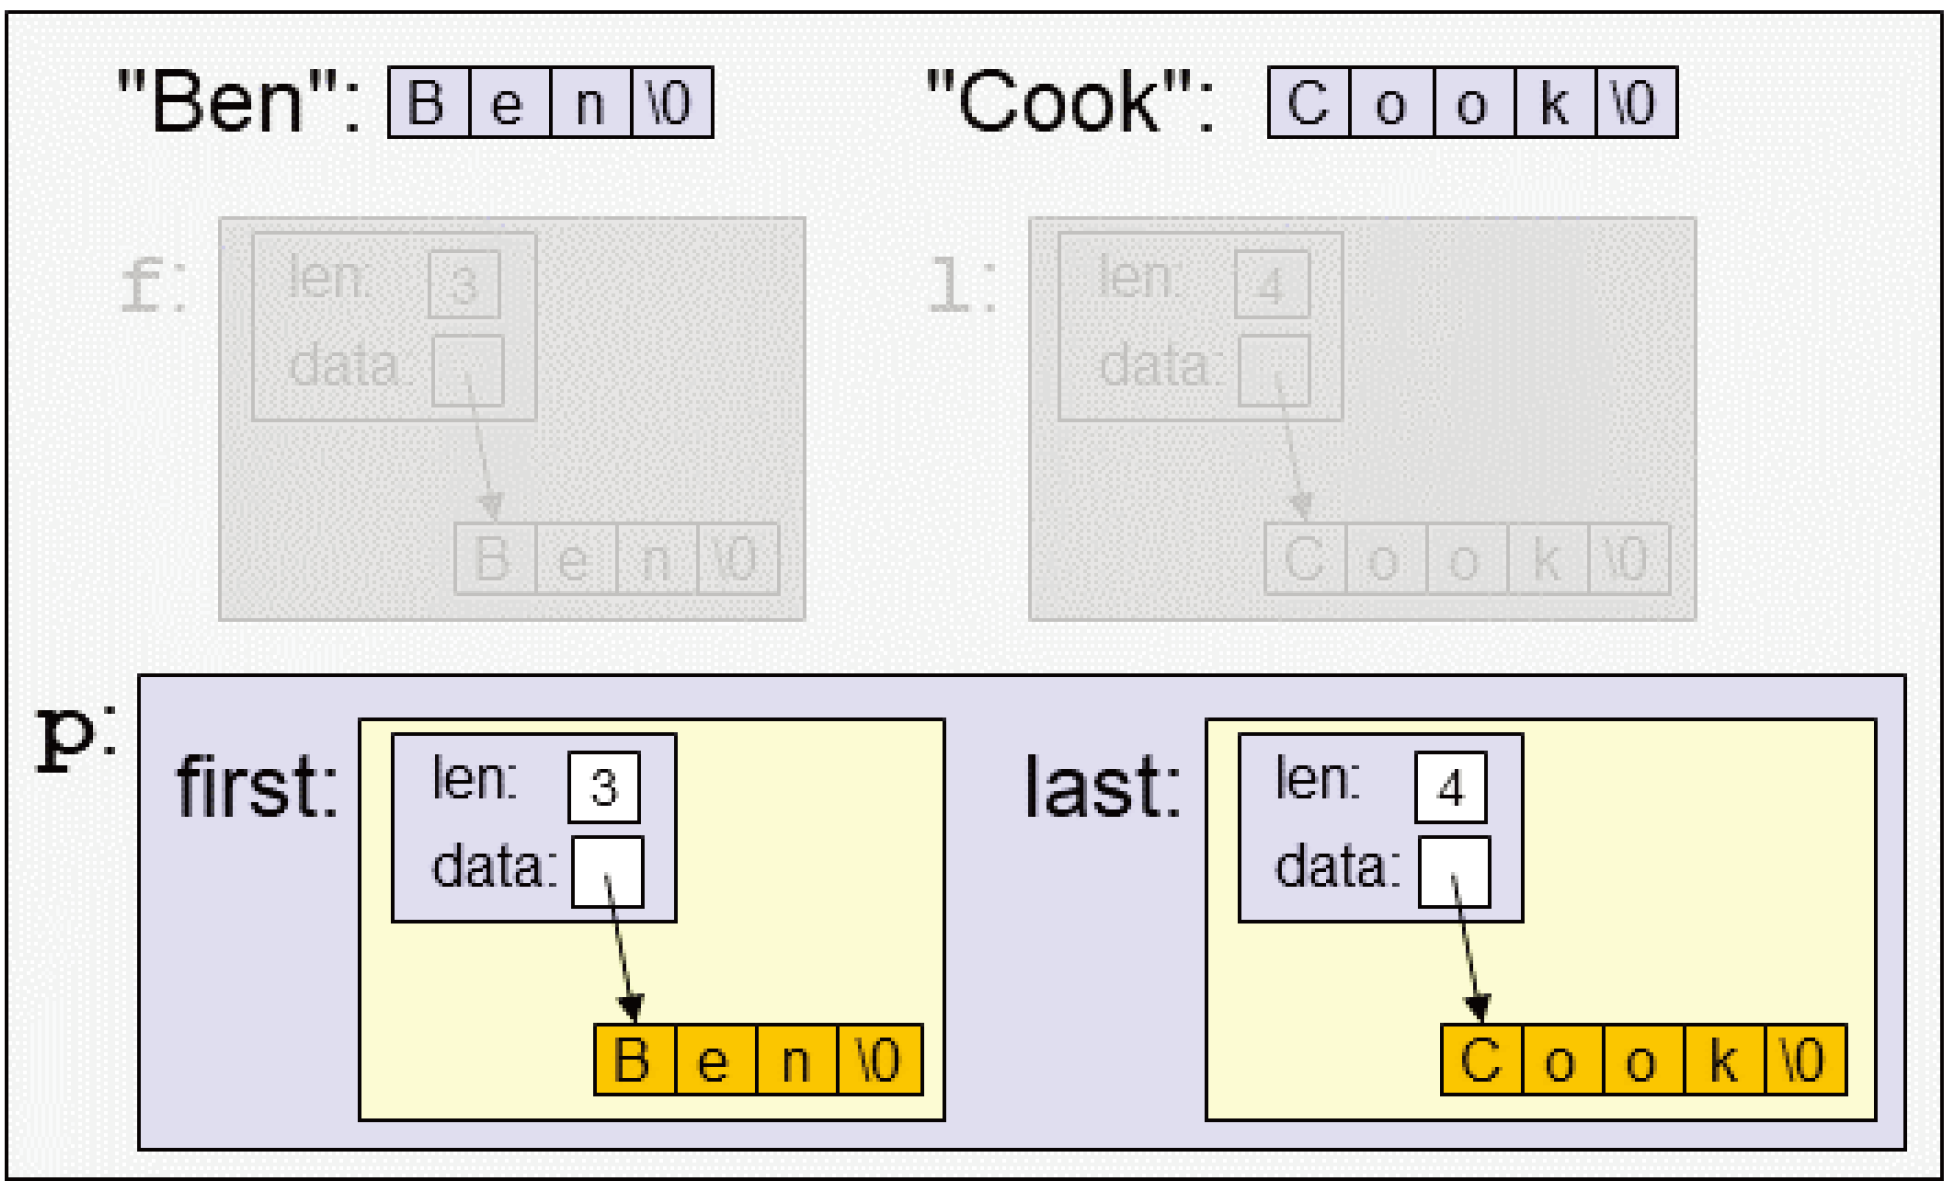
\includegraphics[width=0.6\textwidth]{content/1/chapter4/images/3}
\end{center}

这意味着我们有四个内存分配,尽管只有两个是必要的。所以,使用移动语义的话可以做得更好。\par

\hspace*{\fill} \par %插入空行
\textbf{使用非const左值引用?}

你可能想知道为什么这里不能简单地使用非const左值引用:\par

\begin{lstlisting}[caption={}]
class Person {
	...
	Person(std::string& f, std::string& l)
	: first{std::move(f)}, last{std::move(l)} {
	}
	...
};
\end{lstlisting}

但是,传递const std::string和临时对象(例如,由类型转换创建的)将无法编译:\par

\begin{lstlisting}[caption={}]
Person p{"Ben", "Cook"}; // ERROR: cannot bind a non-const lvalue reference to a temporary
\end{lstlisting}

通常,非const左值引用不会绑定到临时对象。因此,这个构造函数不能将f和l绑定到由字面值创建的临时字符串。\par

\hspace*{\fill} \par %插入空行
\textbf{4.3.2 通过移动参数的值初始化成员}

有了移动语义,构造函数就有了一种简单的初始化成员的方法:构造函数按值接受每个参数,并将其移动到成员中:\par

{\color{red}{basics/initmove.hpp}}

\begin{lstlisting}[caption={}]
#include <string>
class Person {
private:
	std::string first; // first name
	std::string last; // last name
public:
	Person(std::string f, std::string l)
	: first{std::move(f)}, last{std::move(l)} {
	}
	...
};
\end{lstlisting}

这个构造函数接受所有可能的参数,并确保每个参数只有一个分配。\par

例如,如果传递两个字符串的字面值:\par

\begin{lstlisting}[caption={}]
Person p{"Ben", "Cook"};
\end{lstlisting}

我们首先使用它们来初始化参数f和l:\par

\begin{center}
	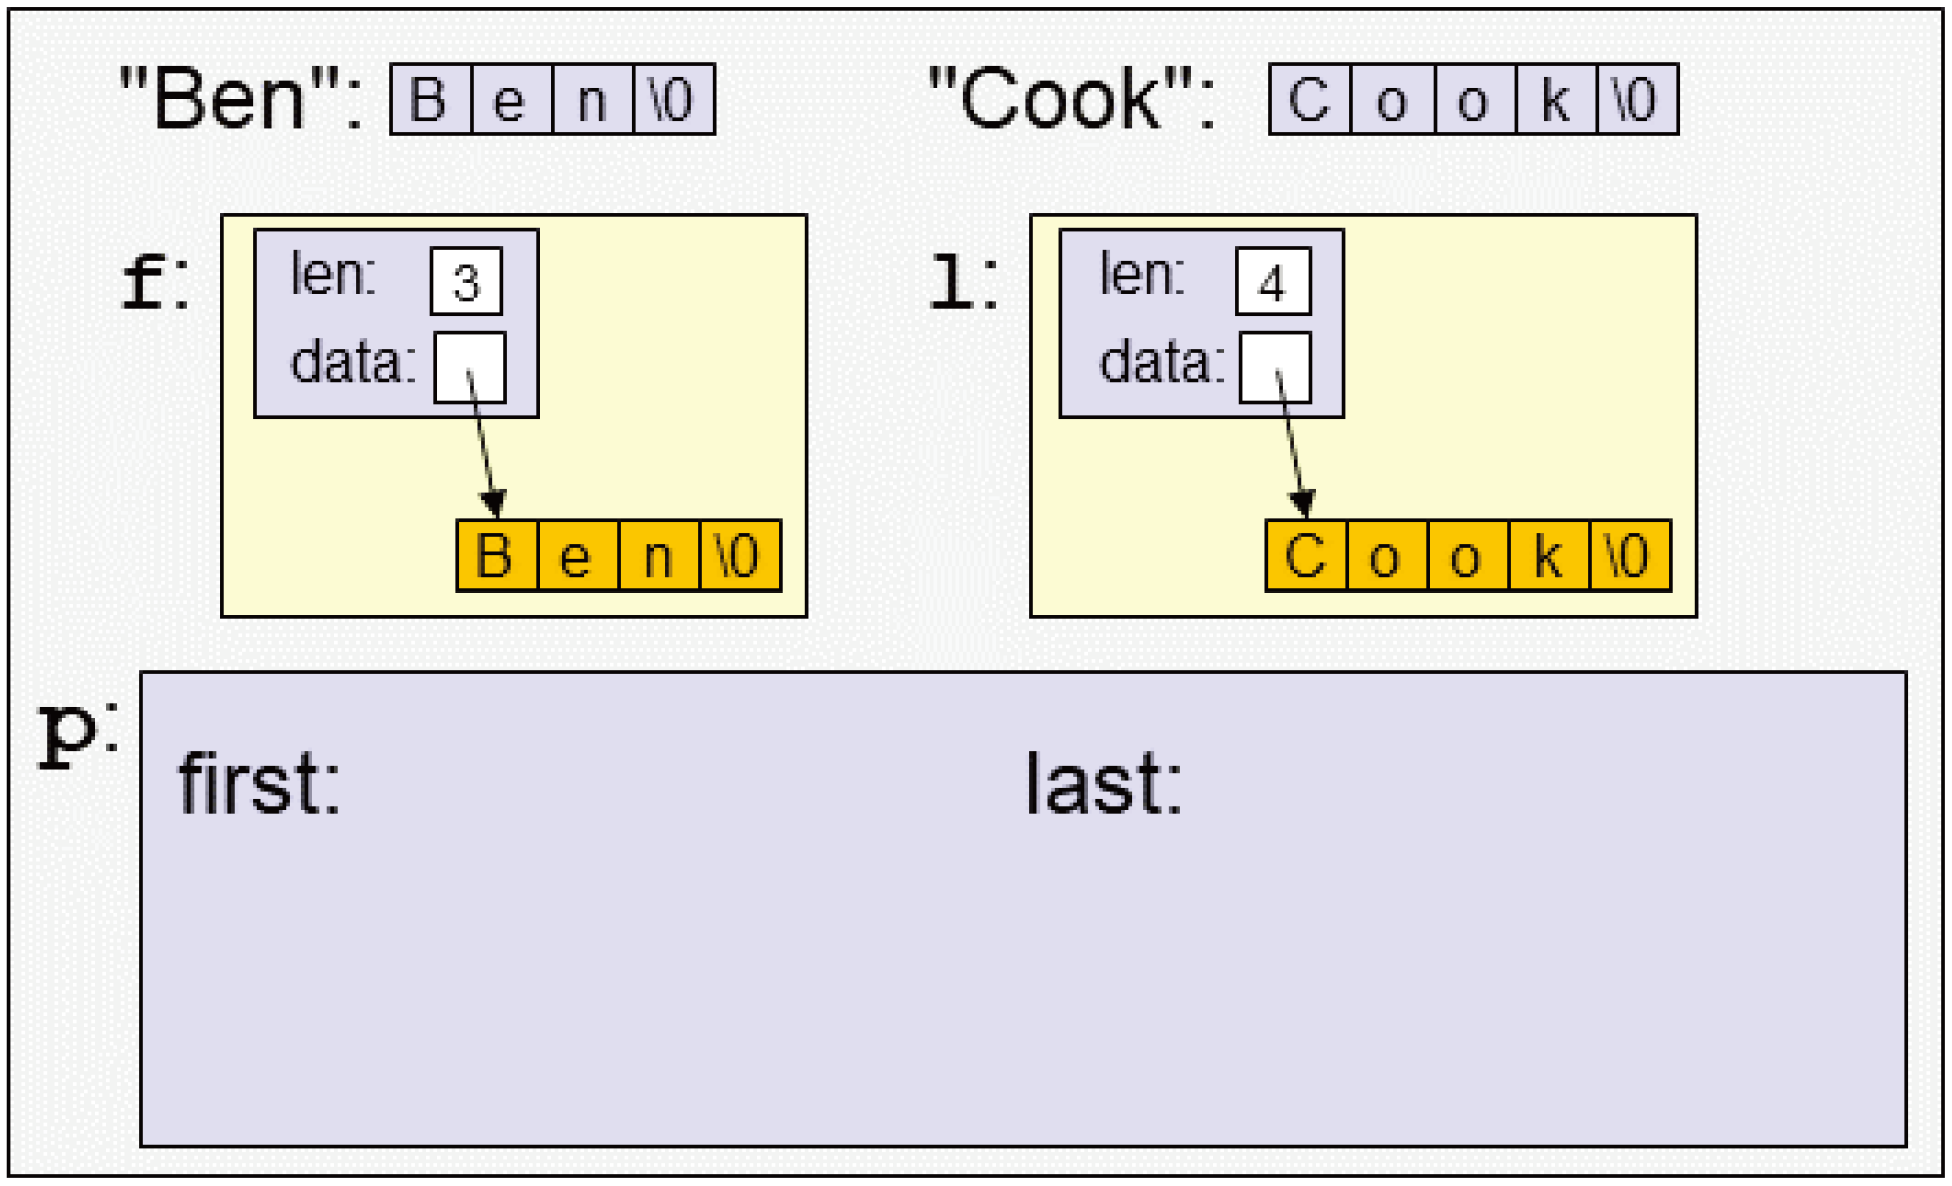
\includegraphics[width=0.6\textwidth]{content/1/chapter4/images/4}
\end{center}

通过使用\textit{std::move()},可以将形参的值移动到成员中。首先,成员首先从f中窃取值:\par

\begin{center}
	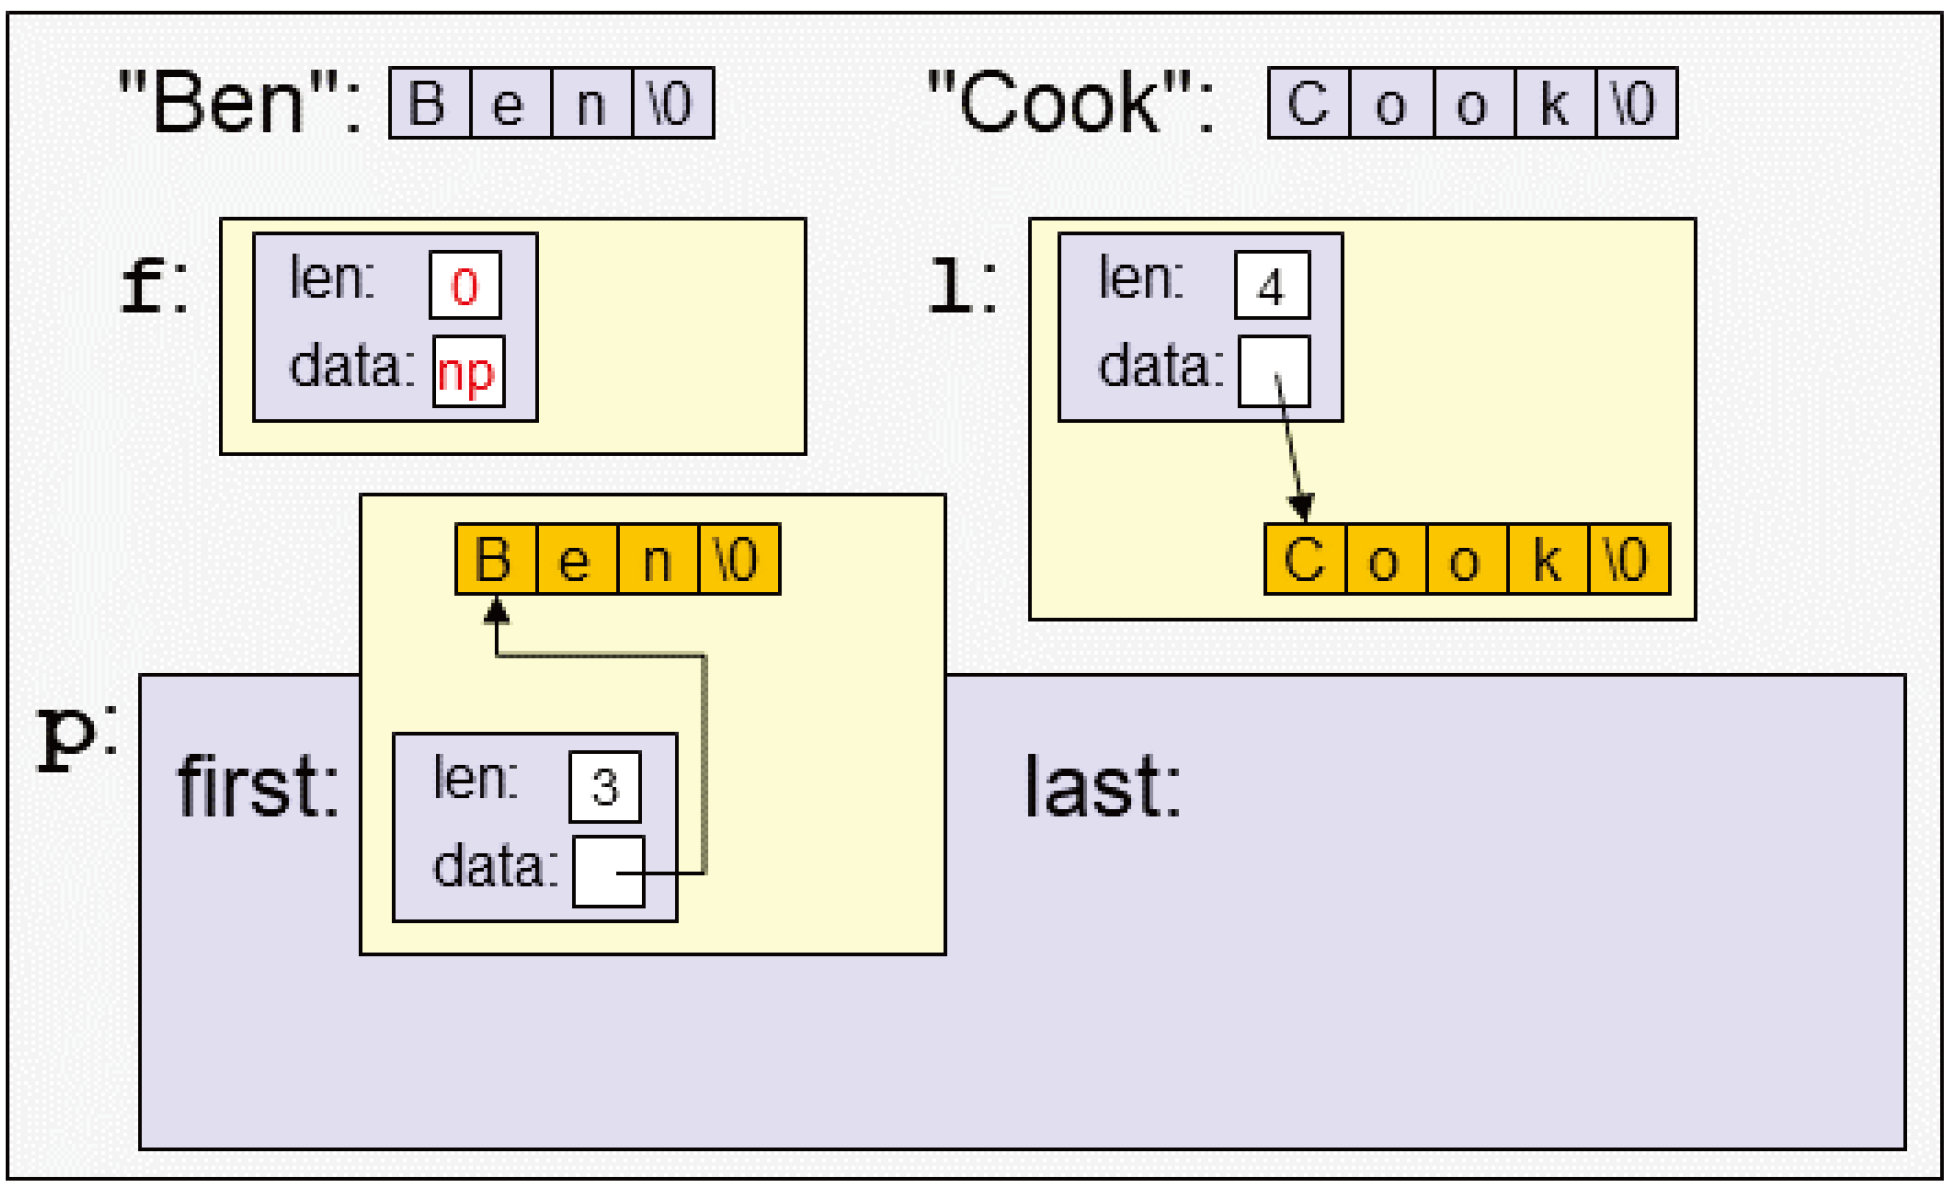
\includegraphics[width=0.6\textwidth]{content/1/chapter4/images/5}
\end{center}

然后,成员last从l中窃取值:\par

\begin{center}
	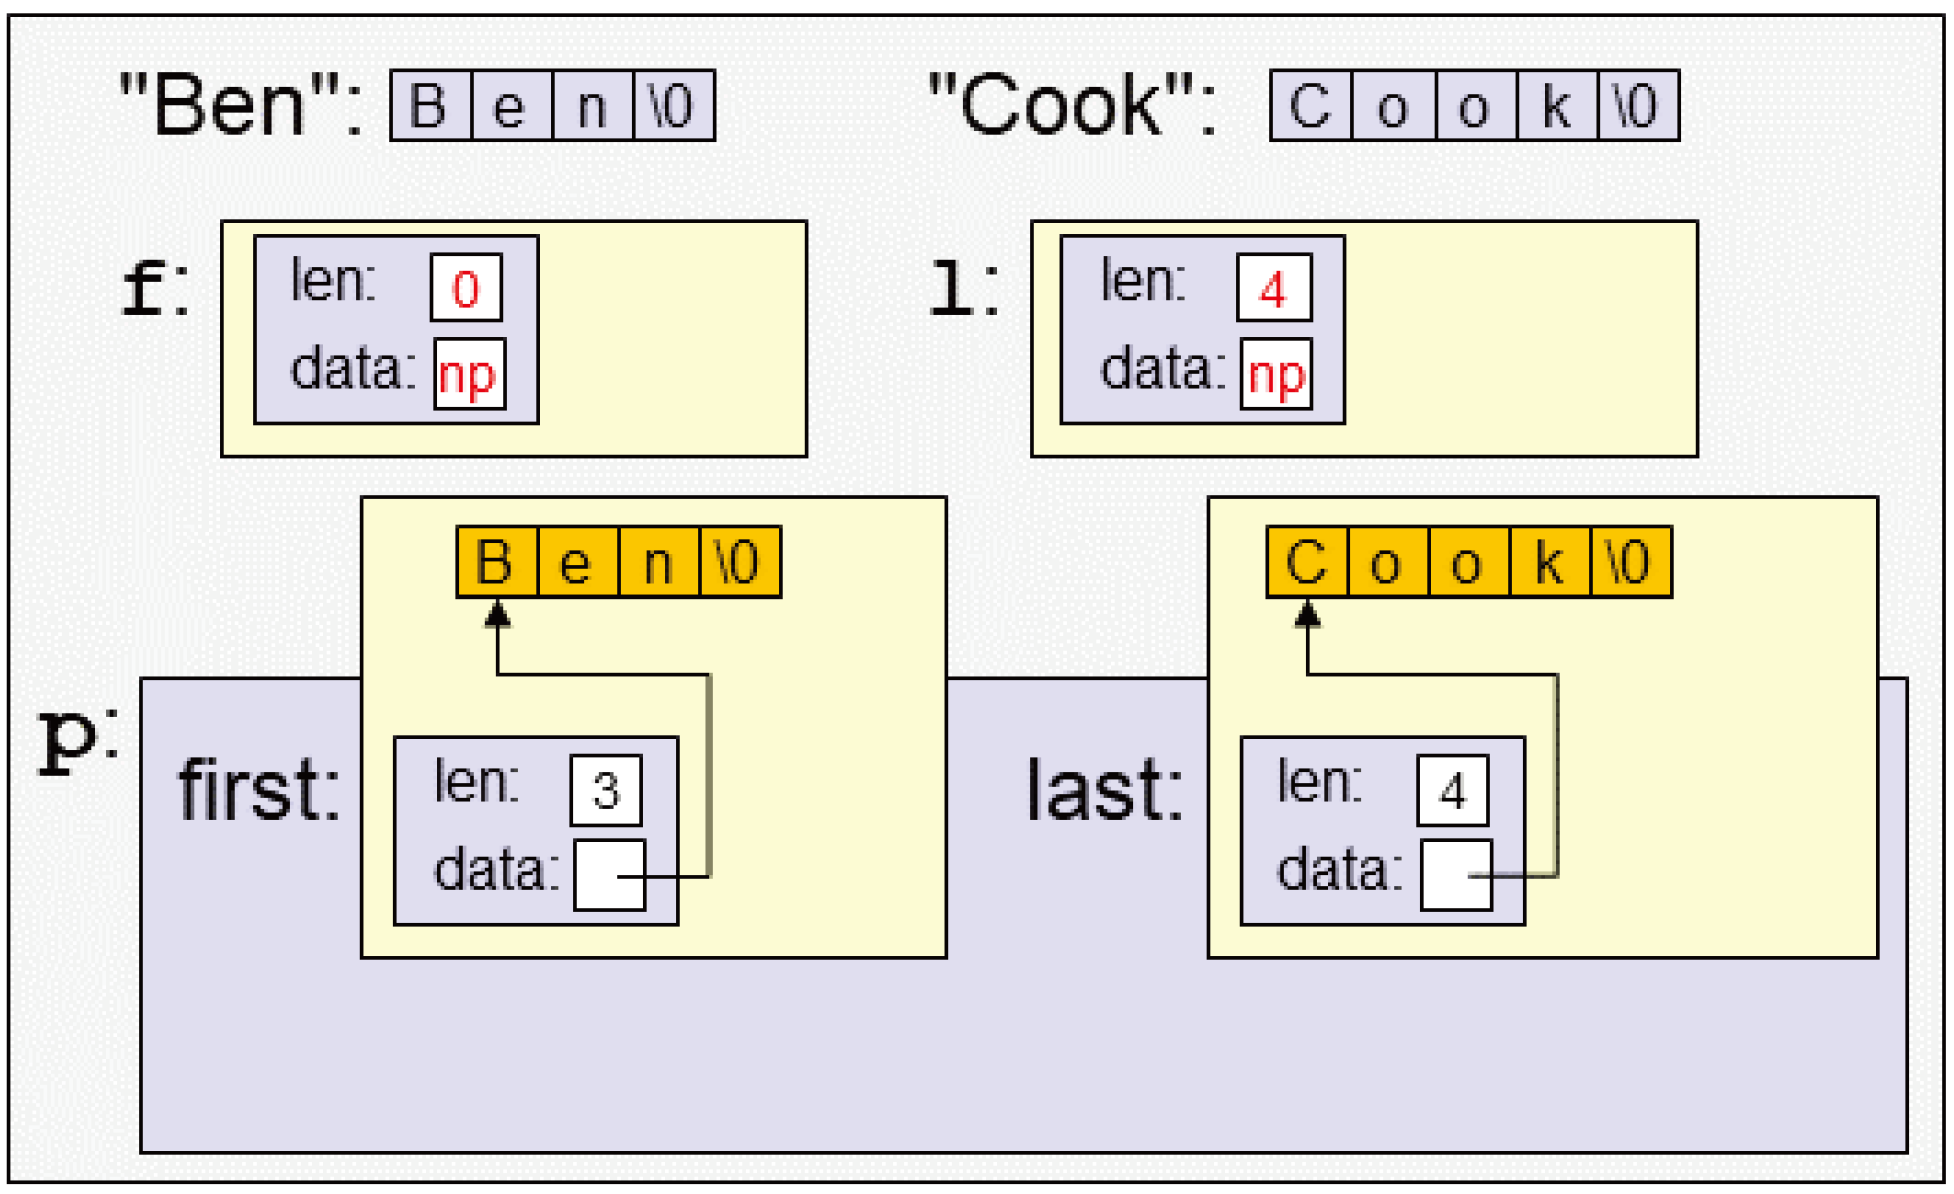
\includegraphics[width=0.6\textwidth]{content/1/chapter4/images/6}
\end{center}

同样,在构造函数的末尾,销毁临时字符串。这一次它花费的时间更少,因为字符串的析构函数不再需要释放分配的内存:\par

\begin{center}
	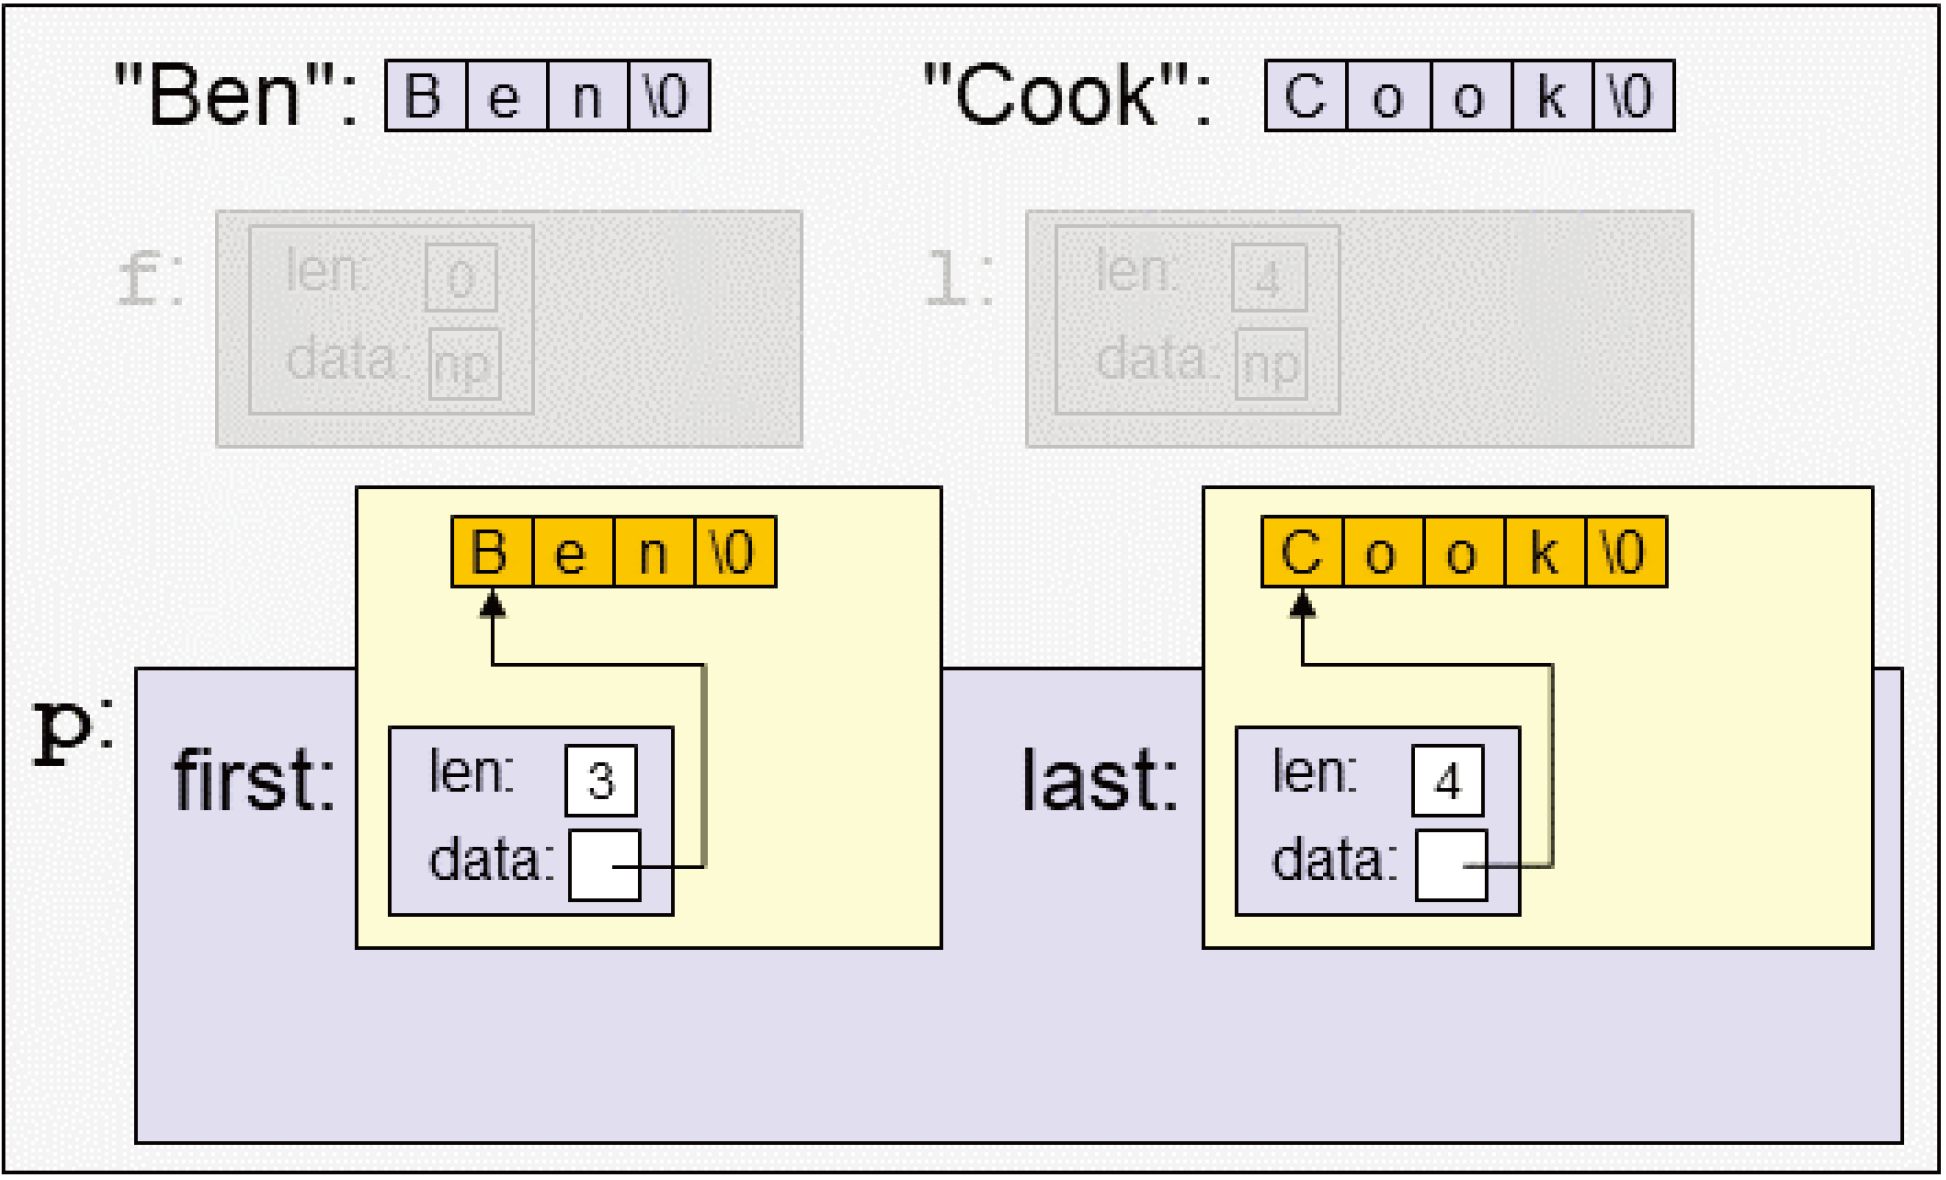
\includegraphics[width=0.6\textwidth]{content/1/chapter4/images/7}
\end{center}

如果传入std::strings,这种初始化成员的方式也能正常工作:\par

\begin{itemize}
	\item 如果传递两个现有字符串而不使用\textit{std::move()}标记,则将名称复制到形参中,并将它们移动到成员中:\par
	\begin{lstlisting}[caption={}]
	std::string name1{"Jane"}, name2{"White"};
	...
	Person p{name1, name2}; // OK, copy names into parameters and move them to the members
	\end{lstlisting}
	\item 如果传递两个不再需要该值的字符串,则根本不需要任何内存分配:
	\begin{lstlisting}[caption={}]
	std::string firstname{"Jane"};
	...
	Person p{std::move(firstname), // OK, move names via parameters to members
		getLastnameAsString()};
	\end{lstlisting}
	本例中,移动了传递的字符串两次:一次是初始化参数f和l,另一次是将f和l的值移动到成员。
\end{itemize}

如果移动很廉价,那么在只有一个构造函数的实现时,任何初始化都是可能的和廉价的。\par

\hspace*{\fill} \par %插入空行
\textbf{4.3.3 通过右值引用初始化成员}

还有更多的方法可以初始化Person的成员,使用多个构造函数。\par

\hspace*{\fill} \par %插入空行
\textbf{使用右值引用}

为了支持移动语义,已经了解了可以将形参声明为非const右值引用。这允许参数从传递的临时对象或标记为\textit{std::move()}的对象中窃取值。\par

考虑这样声明的构造函数:\par

\begin{lstlisting}[caption={}]
class Person {
	...
	Person(std::string&& f, std::string&& l)
	: first{std::move(f)}, last{std::move(l)} {
	}
	...
};
\end{lstlisting}

这个初始化也适用于我们传递的字符串:\par

\begin{lstlisting}[caption={}]
Person p{"Ben", "Cook"};
\end{lstlisting}

同样,因为构造函数需要字符串,我们创建f和l绑定的两个临时字符串:\par

\begin{center}
	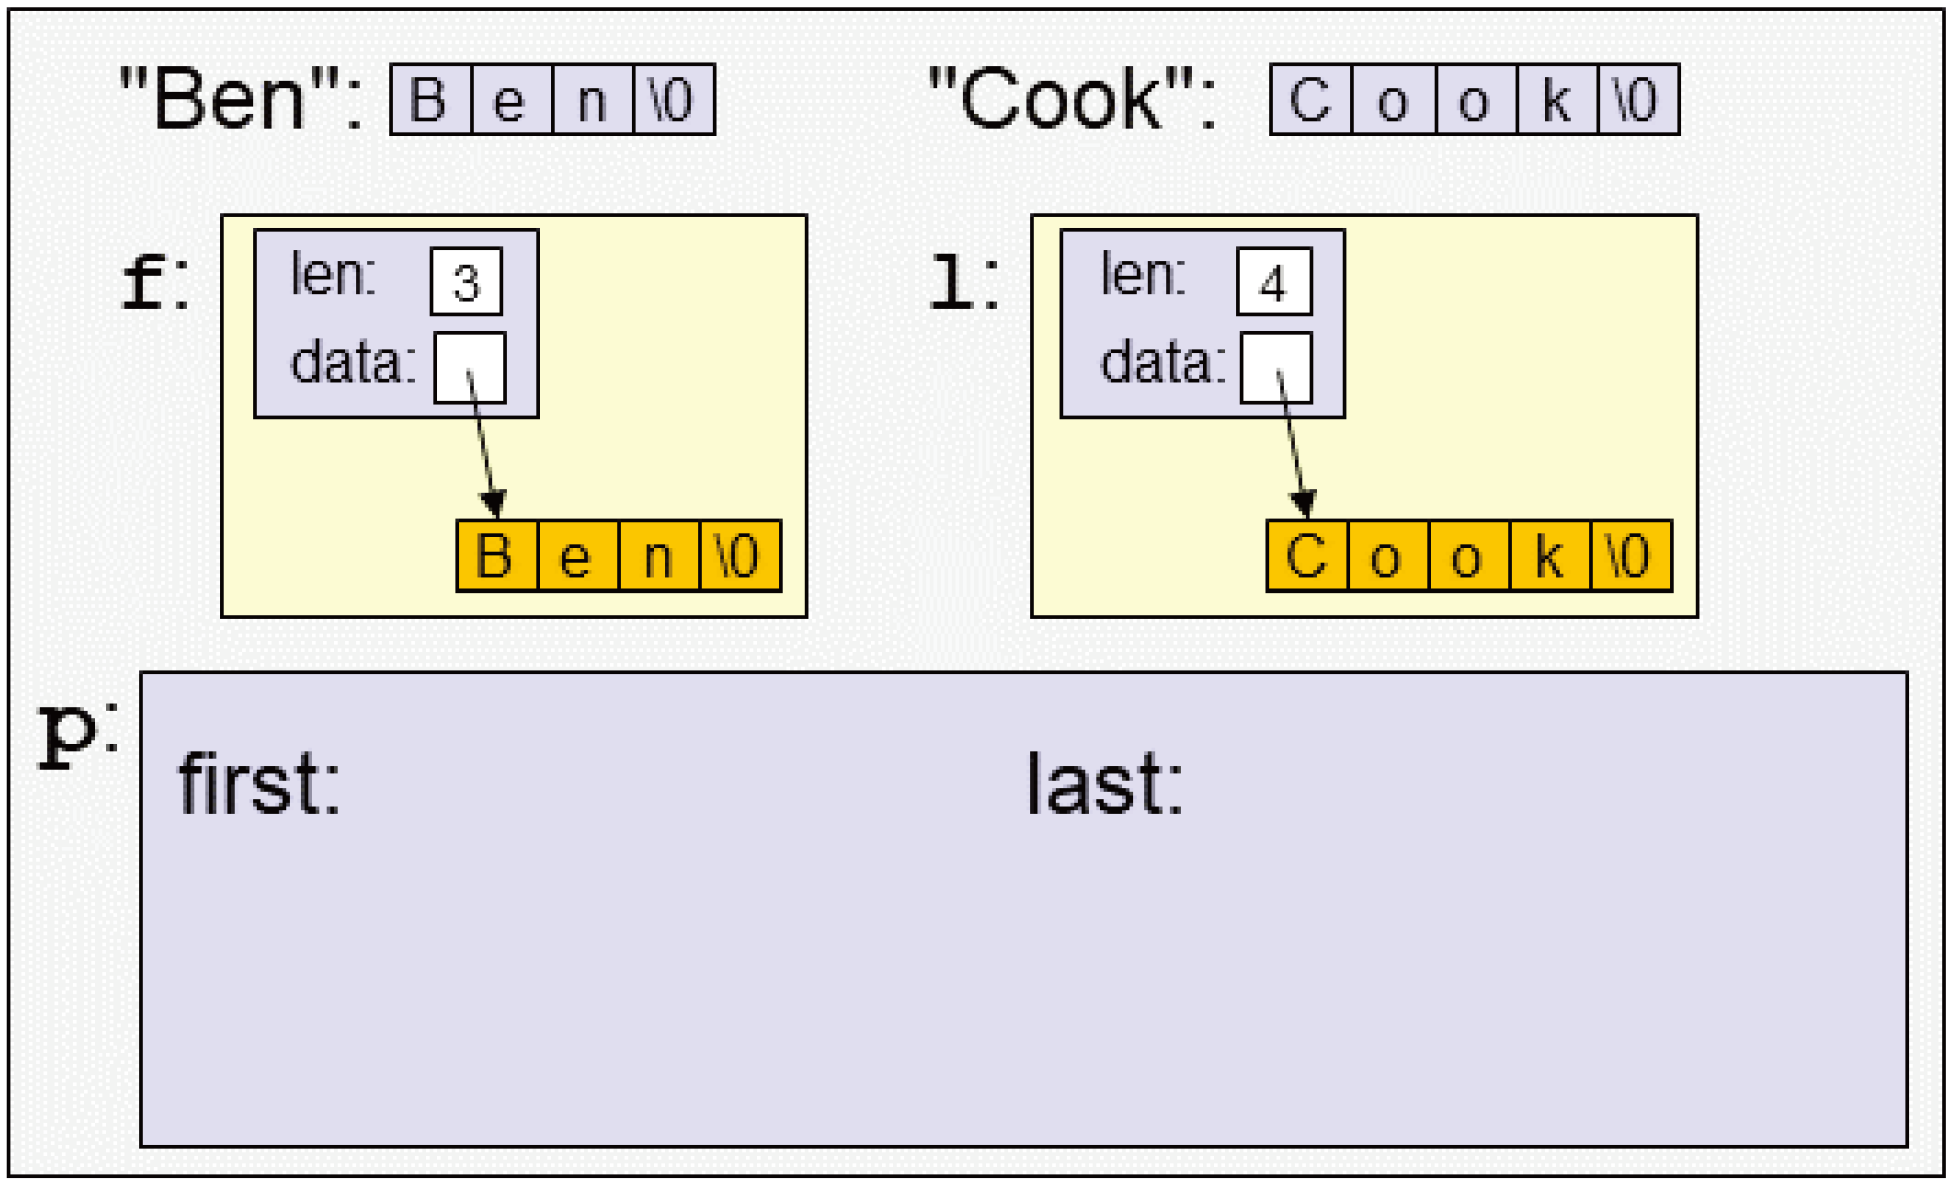
\includegraphics[width=0.6\textwidth]{content/1/chapter4/images/8}
\end{center}

因为有非const引用,所以可以修改。本例中,用\textit{std::move()}标记它们,以便成员的初始化可以窃取值。\par

首先,成员首先从f中窃取值:\par

\begin{center}
	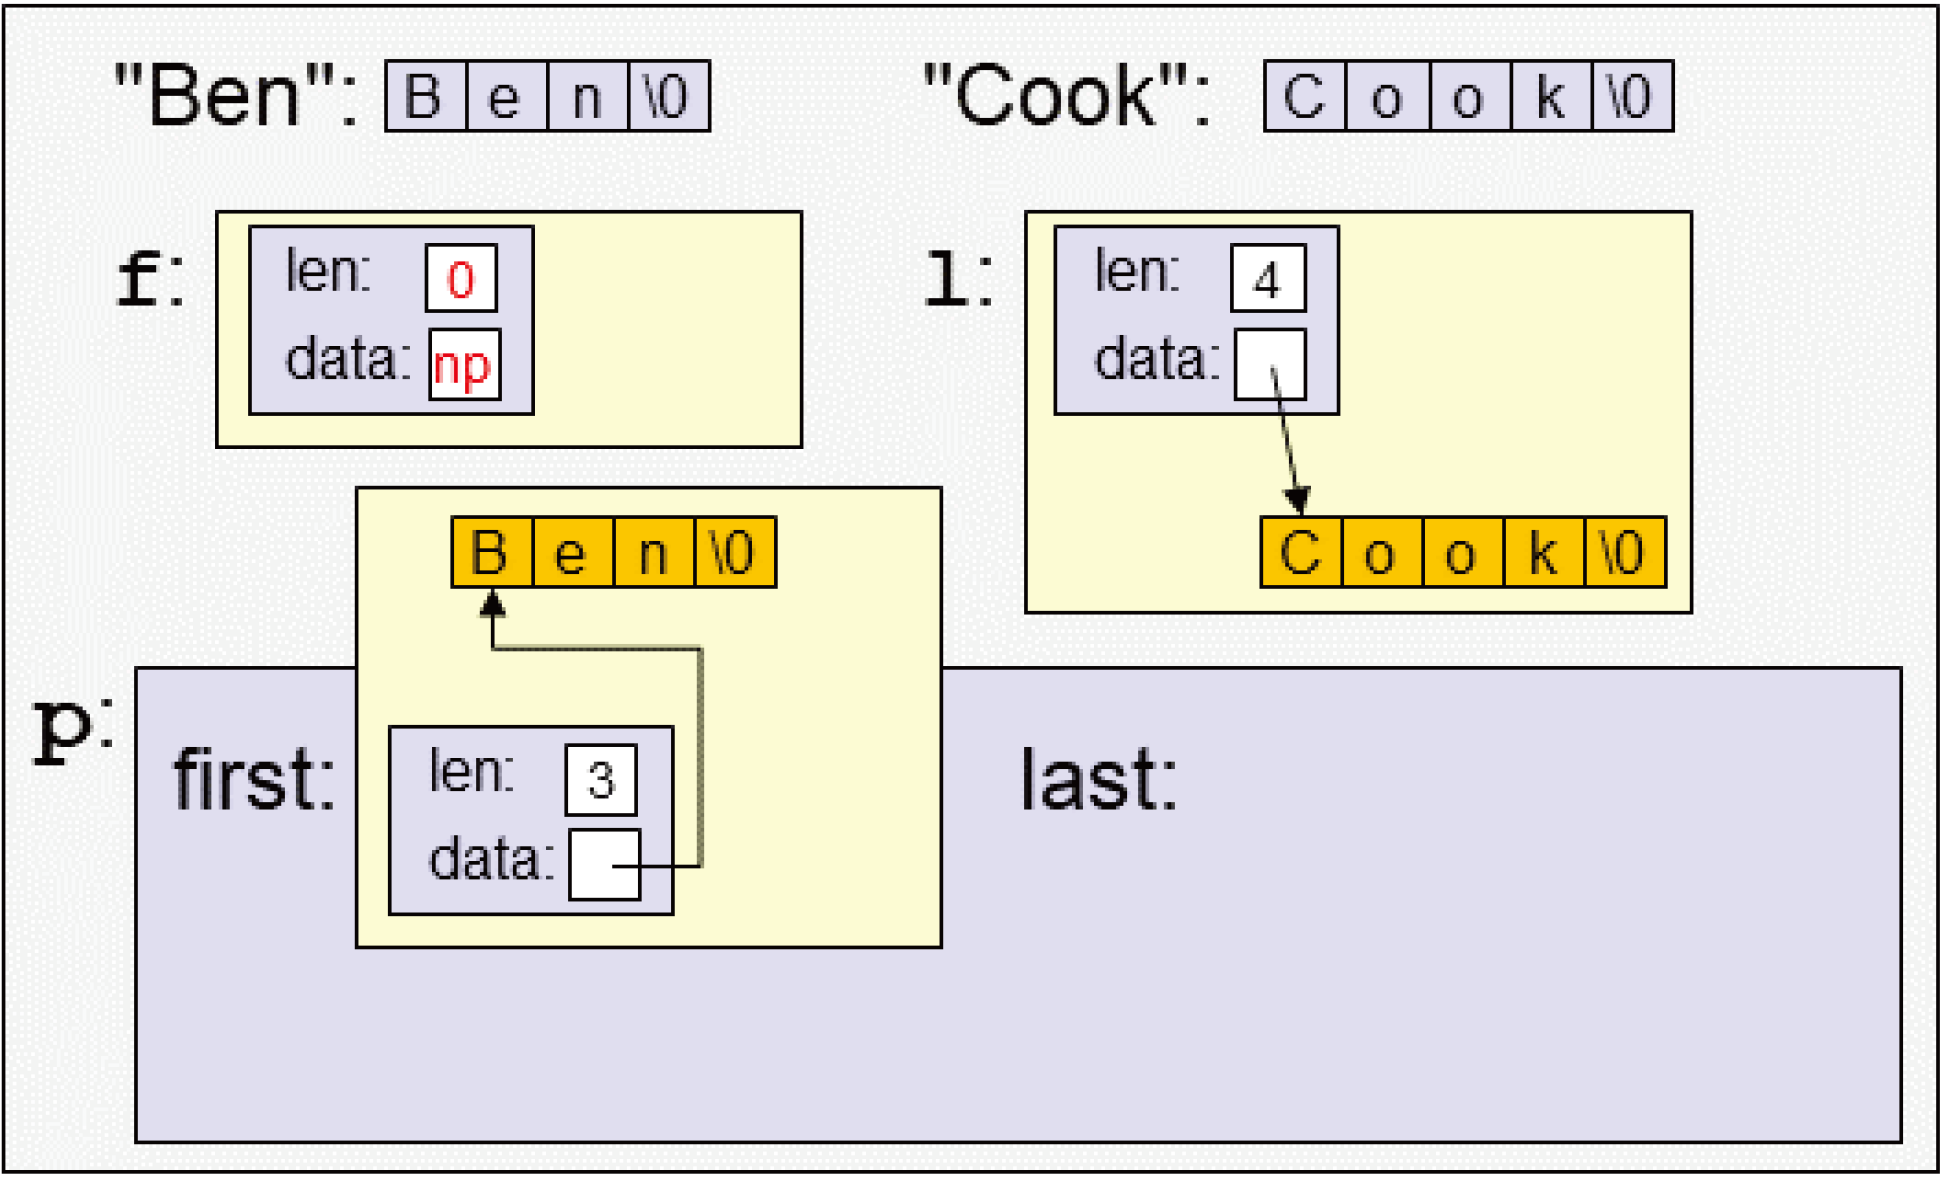
\includegraphics[width=0.6\textwidth]{content/1/chapter4/images/9}
\end{center}

然后,成员last从l中窃取值:\par

\begin{center}
	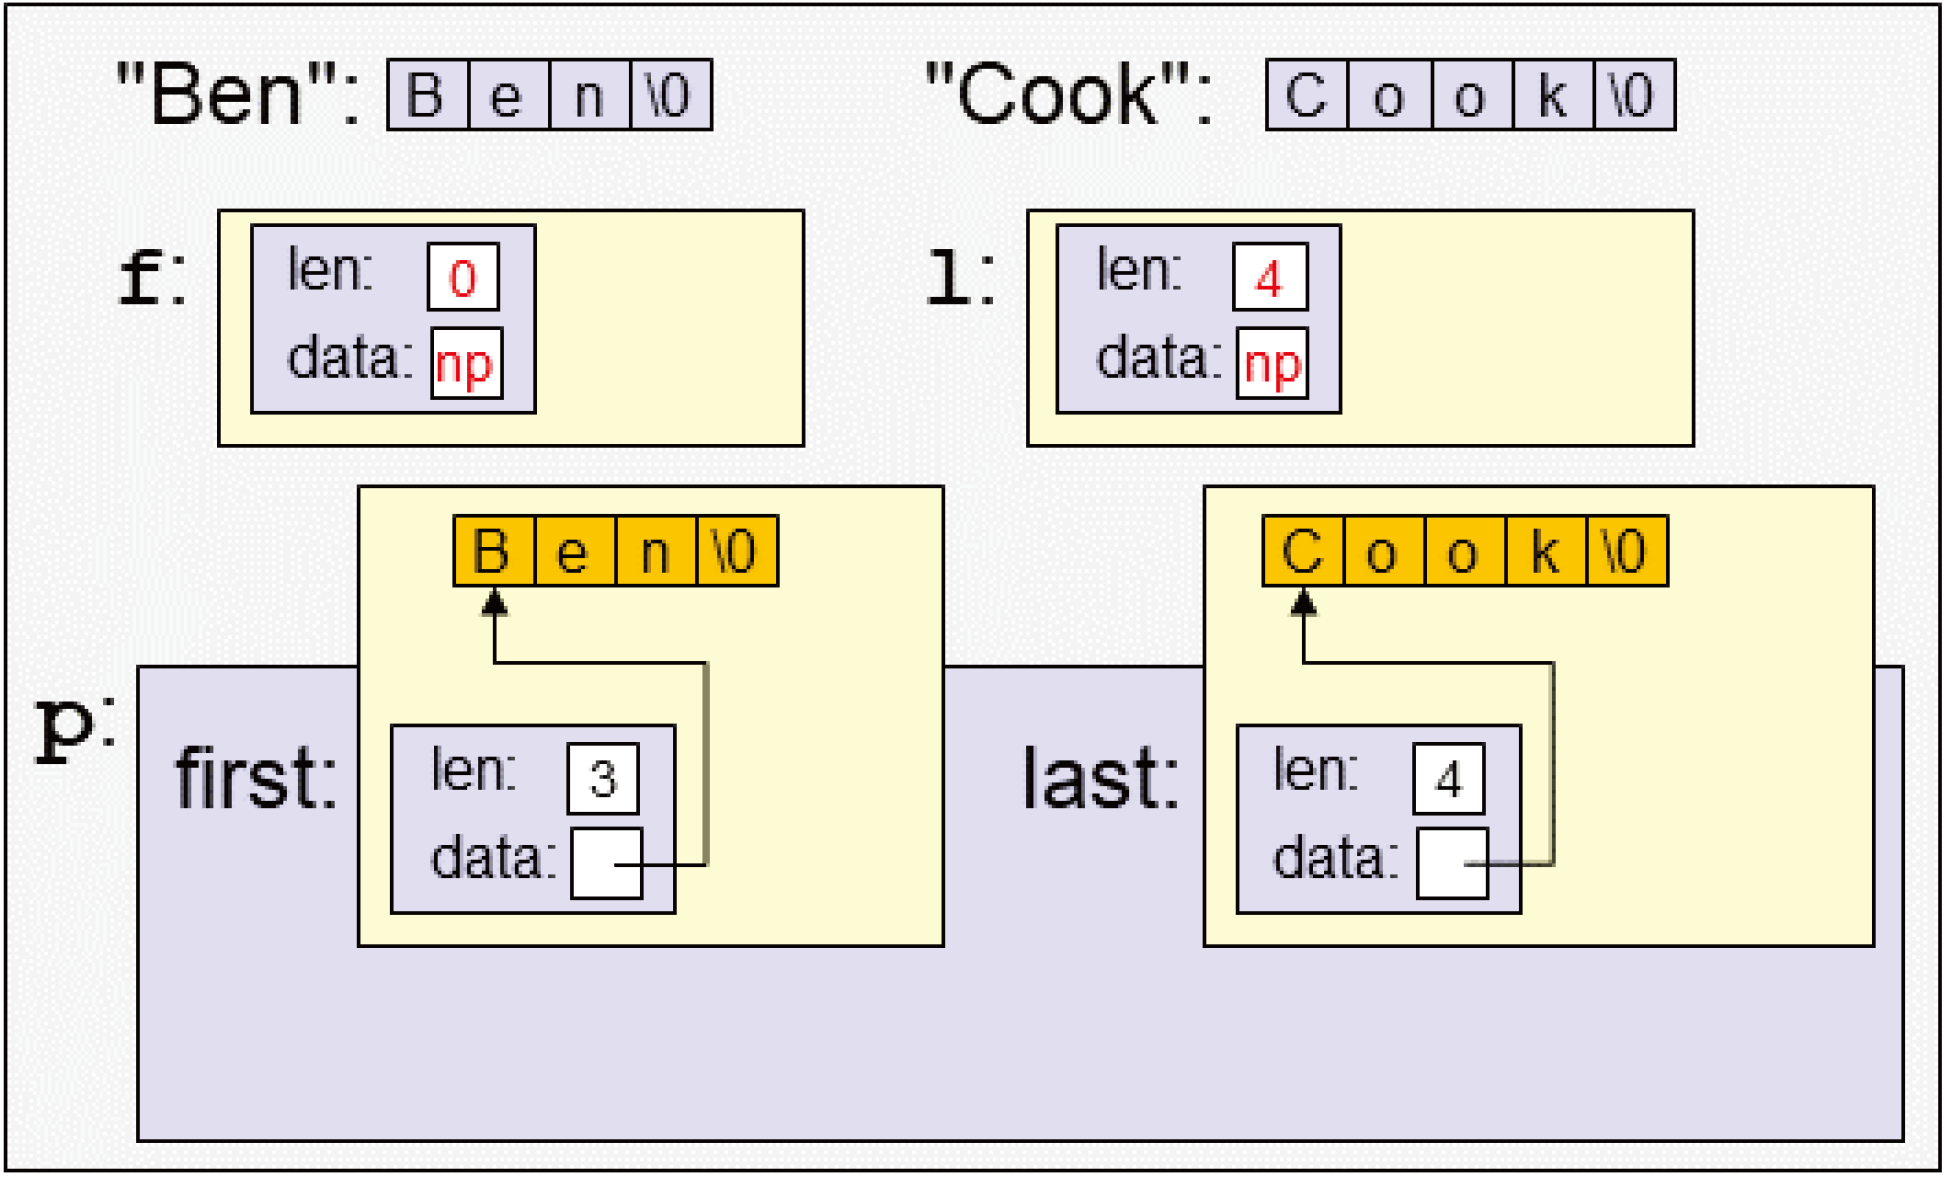
\includegraphics[width=0.6\textwidth]{content/1/chapter4/images/10}
\end{center}

同样,在构造函数的末尾,销毁临时字符串而不需要释放已分配的内存:\par

\begin{center}
	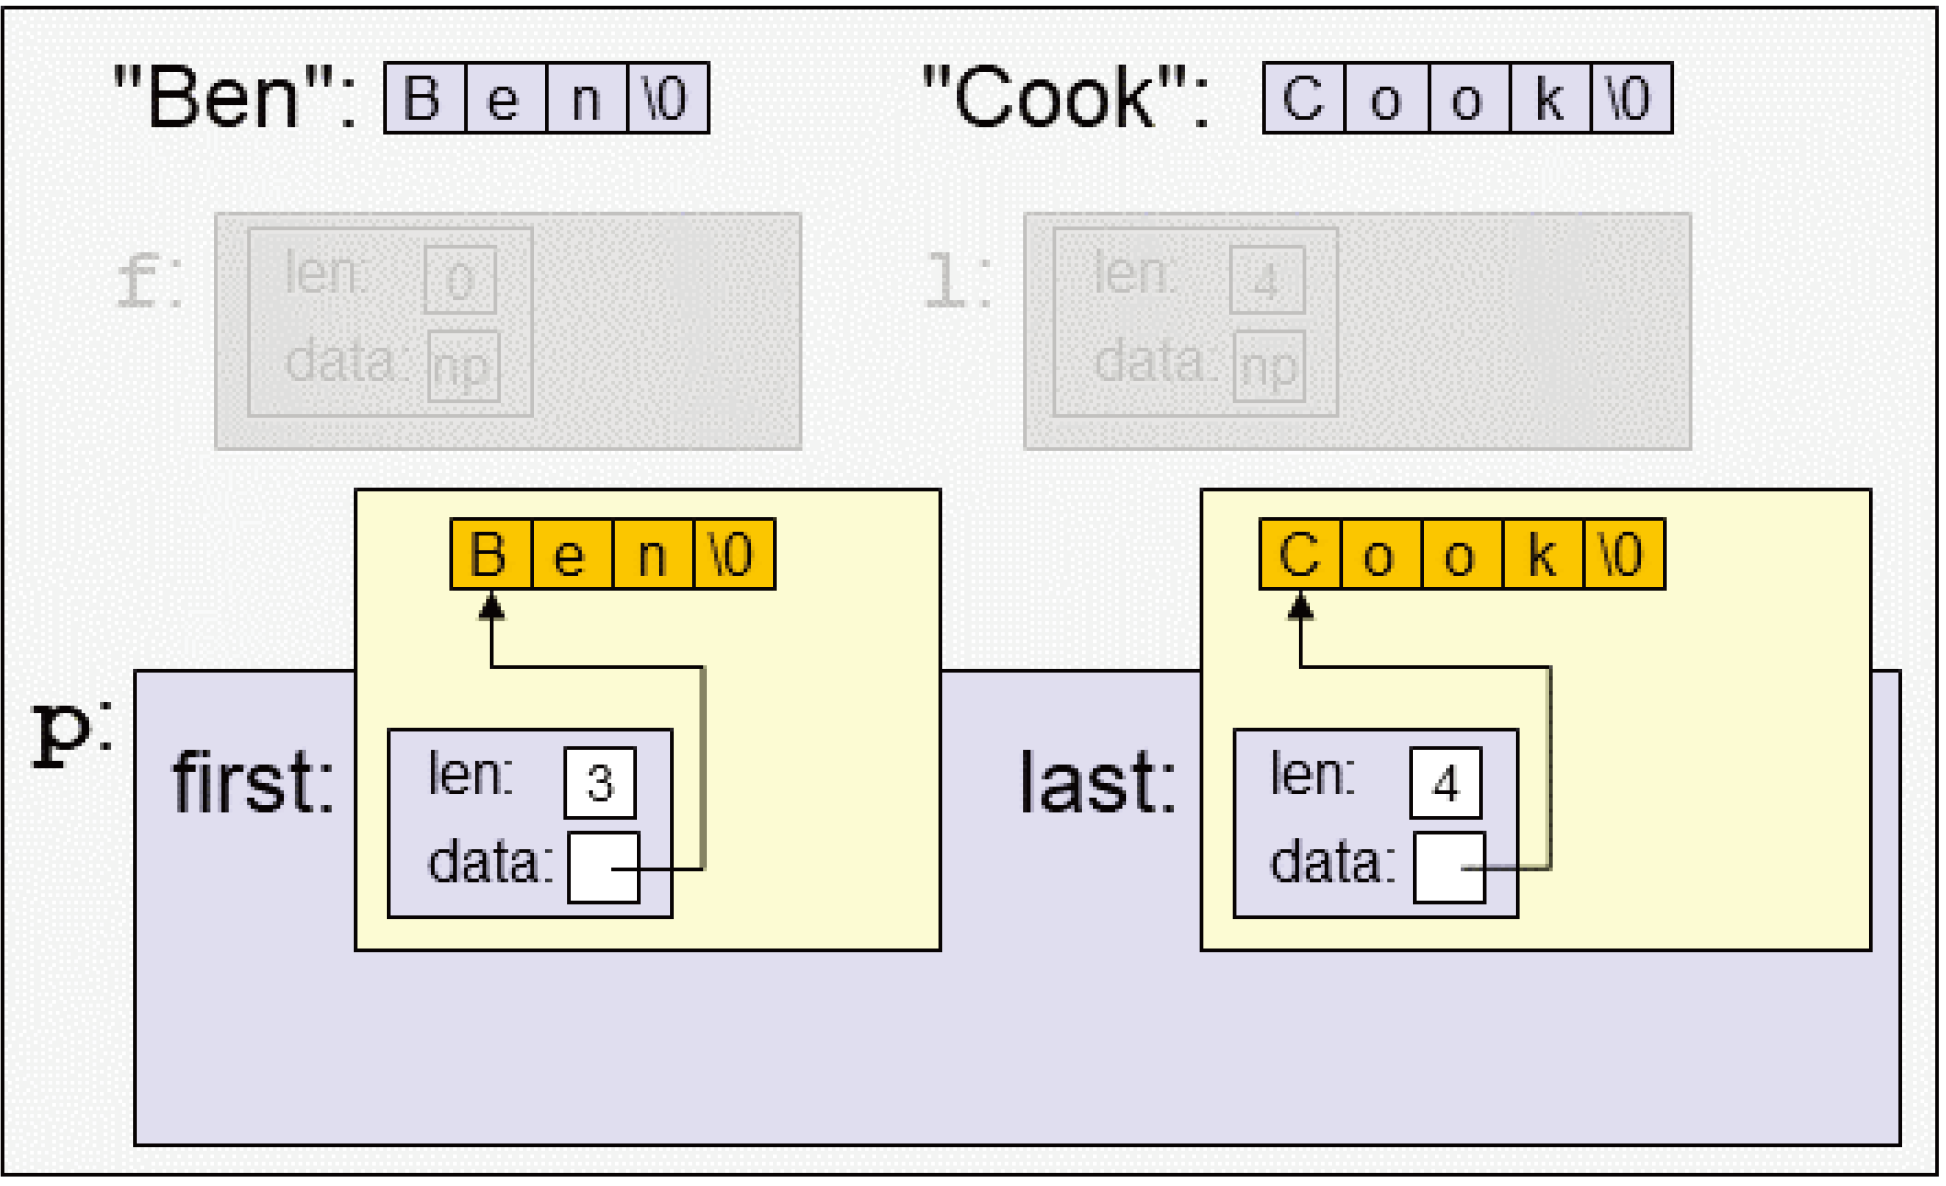
\includegraphics[width=0.6\textwidth]{content/1/chapter4/images/11}
\end{center}

然而,此构造函数并非在所有情况下都有效。\par

\hspace*{\fill} \par %插入空行
\textbf{重载右值和左值引用}

虽然右值引用的函数在传递临时对象时,工作得很好(传递由字符串字面值创建的临时std::string),但它们也有限制:不能传递之后还需要值的已命名对象。因此,如果只有一个接受右值引用的构造函数,就不能传递现有的字符串:\par

\begin{lstlisting}[caption={}]
class Person {
	...
	Person(std::string&& f, std::string&& l)
	: first{std::move(f)}, last{std::move(l)} {
	}
	...
};

Person p1{"Ben", "Cook"}; // OK

std::string name1{"Jane"}, name2{"White"};
...
Person p2{name1, name2}; // ERROR: can’t pass a named object to an rvalue reference
\end{lstlisting}

对于p2,我们需要一个传统的构造函数,使用const左值引用声明。然而,也可以传递一个字符串字面值和一个现有的字符串。因此,总共需要四个构造函数来处理所有可能的组合:\par

\begin{lstlisting}[caption={}]
class Person {
	...
	Person(const std::string& f, const std::string& l)
	: first{f}, last{l} {
	}
	Person(const std::string& f, std::string&& l)
	: first{f}, last{std::move(l)} {
	}
	Person(std::string&& f, const std::string& l)
	: first{std::move(f)}, last{l} {
	}
	Person(std::string&& f, std::string&& l)
	: first{std::move(f)}, last{std::move(l)} {
	}
	...
};
\end{lstlisting}

这样,我们可以以任意组合传递字符串字面值和现有字符串,而且每个成员总是只有一个分配。\par

\hspace*{\fill} \par %插入空行
\textbf{重载字符串字面值}

为了进一步提高性能,我们甚至可能有特定的实现,将字符串文字作为普通指针。这样的话,我们甚至可以避免一些动作。然而,实现所有构造函数有点乏味:\par

{\color{red}{basics/initall.hpp}}

\begin{lstlisting}[caption={}]
#include <string>
class Person {
	private:
	std::string first; // first name
	std::string last; // last name
	public:
	Person(const std::string& f, const std::string& l)
	: first{f}, last{l} {
	}
	Person(const std::string& f, std::string&& l)
	: first{f}, last{std::move(l)} {
	}
	Person(std::string&& f, const std::string& l)
	: first{std::move(f)}, last{l} {
	}
	Person(std::string&& f, std::string&& l)
	: first{std::move(f)}, last{std::move(l)} {
	}
	Person(const char* f, const char* l)
	: first{f}, last{l} {
	}
	Person(const char* f, const std::string& l)
	: first{f}, last{l} {
	}
	Person(const char* f, std::string&& l)
	: first{f}, last{std::move(l)} {
	}
	Person(const std::string& f, const char* l)
	: first{f}, last{l} {
	}
	Person(std::string&& f, const char* l)
	: first{std::move(f)}, last{l} {
	}
	...
};
\end{lstlisting}

这个解决方案的好处是减少了移动的次数。如果传递一个字符串字面值,则直接使用传递的指针初始化成员,而不是创建std::string并将其值移动到成员。\par

\hspace*{\fill} \par %插入空行
\textbf{4.3.4 比较不同的方法}

随着初始化成员的新方法的引入,我们应该在什么时候使用哪种技术?\par

通常,应该有一个很好的理由不使用const\&的简单方法。这个原因通常是表现。因此,测量一下使用三种参数初始化person需要多长时间:传递字符串字面值,传递现有字符串,以及传递标有\textit{std::move()}的字符串:\par

\begin{lstlisting}[caption={}]
std::string fname = "a first name";
std::string lname = "a last name";

// measure how long this takes:
Person p1{"a firstname", "a lastname"};
Person p2{fname, lname};
Person p3{std::move(fname), std::move(lname)};
\end{lstlisting}

然而,为了避免小字符串优化(这意味着字符串根本不分配任何内存),我们应该使用具有显著长度的字符串。所以,这里有一个完整的函数来衡量不同的方法:\par

{\color{red}{basics/initmeasure.hpp}}

\begin{lstlisting}[caption={}]
#include <chrono>

// measure num initializations of whatever is currently defined as Person:
std::chrono::nanoseconds measure(int num)
{
	std::chrono::nanoseconds totalDur{0};
	for (int i = 0; i < num; ++i) {
		std::string fname = "a firstname a bit too long for SSO";
		std::string lname = "a lastname a bit too long for SSO";
		
		// measure how long it takes to create 3 Persons in different ways:
		auto t0 = std::chrono::steady_clock::now();
		Person p1{"a firstname too long for SSO", "a lastname too long for SSO"};
		Person p2{fname, lname};
		Person p3{std::move(fname), std::move(lname)};
		auto t1 = std::chrono::steady_clock::now();
		totalDur += t1 - t0;
	}
	return totalDur;
}
\end{lstlisting}

函数measure()返回执行上述三种初始化的num迭代的持续时间,并使用长度够长的字符串。\par

现在,我们将上面类Person的不同定义与measure函数结合起来,并使用main()函数调用measure函数,并打印消耗的时间。例如:\par

{\color{red}{basics/initclassicperf.cpp}}

\begin{lstlisting}[caption={}]
#include "initclassic.hpp"
#include "initmeasure.hpp"
#include <iostream>
#include <cstdlib> // for std::atoi()

int main(int argc, const char** argv)
{
	int num = 1000; // num iterations to measure
	if (argc > 1) {
		num = std::atoi(argv[1]);
	}

	// a few iterations to avoid measuring initial behavior:
	measure(5);
	
	// measure (in integral nano- and floating-point milliseconds):
	std::chrono::nanoseconds nsDur{measure(num)};
	std::chrono::duration<double, std::milli> msDur{nsDur};
	
	// print result:
	std::cout << num << " iterations take: "
	<< msDur.count() << "ms\n";
	std::cout << "3 inits take on average: "
	<< nsDur.count() / num << "ns\n";
}
\end{lstlisting}

另外两个程序, {\color{red}{basics/initallperf.cpp}}和{\color{red}{basics/initmoveperf.cpp}},只需对Person类的其他声明使用不同的头文件即可。

使用三个不同的编译器,在三个不同的平台上运行这段代码的效果如下:\par

\begin{itemize}
	\item 使用经典左值引用(const \&)的初始化比其他初始化花费的时间要多得多。差不多是其他的2倍时间。
	\item 实现所有9个构造函数与只接受参数值和移动的构造函数之间没有很大区别。
\end{itemize}

如果通过使用非常短的字符串从小字符串优化(SSO)中受益,这意味着我们根本不分配任何内存(并且移动语义应该没有显著帮助),那么耗时是非常接近的。然而,使用接受const左值引用的传统构造函数仍然有一点缺点。\par

除了尝试不同的测试程序,还可以使用{\color{red}{basics/initperf.cpp}}作为一个组合程序,在其他的平台上执行所有测试。\par

然而,你可能有非常大型的成员不能从移动语义中获益(例如一个包含10000个双精度值的数组):\par
 
\begin{lstlisting}[caption={}]
class Person {
private:
	std::string name;
	std::array<double, 10000> values; // move can’t optimize here
public:
	...
};
\end{lstlisting}

在这种情况下,会遇到一个问题:将初始参数的值乘以10000倍,然后移动。我们必须复制参数两次,这几乎需要两倍的时间。请参见{\color{red}{basics/initbigper .cpp}},以获得一个完整的程序示例。\par

\hspace*{\fill} \par %插入空行
\textbf{4.3.5 成员初始化总结}

总的来说,要初始化移动语义对其有显著影响的成员(字符串、容器或具有此类成员的类/数组),你应该在以下选项上使用移动语义:\par

\begin{itemize}
	\item 从通过左值引用获取形参切换到通过值获取形参并将其移动到成员中
	\item 重载移动语义的构造函数
\end{itemize}

第一个选项允许我们只有一个构造函数,这样代码更容易维护。然而,这确实会导致不必要的移动操作。因此,如果移动操作可能花费大量时间,最好使用多个重载。\par

例如,如果有一个带有字符串和值向量的类,按值和移动通常是正确的方法:\par

\begin{lstlisting}[caption={}]
class Person {
private:
	std::string name;
	std::vector<std::string> values;
public:
	Person(std::string n, std::vector<std::string> v)
	: name{std::move(n)}, values{std::move(v)} {
	}
	...
};
\end{lstlisting}

但是,如果有std::array成员,最好重载,因为即使移动了成员,移动std::array也要花费大量的时间:\par

\begin{lstlisting}[caption={}]
class Person {
private:
	std::string name;
	std::array<std::string, 1000> values;
public:
	Person(std::string n, const std::array<std::string, 1000>& v)
	: name{std::move(n)}, values{v} {
	}
	Person(std::string n, std::array<std::string, 1000>&& v)
	: name{std::move(n)}, values{std::move(v)} {
	}
	...
};
\end{lstlisting}

\hspace*{\fill} \par %插入空行
\textbf{4.3.6 总要使用移动进行值传递吗?}

上面的讨论引出了这样一个问题:我们现在是否应该总是按值接受参数,并将它们移动来设置内部值或成员。答案是否定的。\par

这里讨论的特殊情况是创建并初始化一个新值。在这种情况下,这种策略获得了回报。如果已经有一个值,需要对其进行更新或修改,那么使用这种方法将适得其反。\par

一个简单的例子是setter。考虑类Person的以下实现:\par

\begin{lstlisting}[caption={}]
class Person {
private:
	std::string first; // first name
	std::string last; // last name
public:
	Person(std::string f, std::string l)
	: first{std::move(f)}, last{std::move(l)} {
	}
	...
	void setFirstname(std::string s) { // take by value
		first = std::move(s); // and move
	}
	...
};
\end{lstlisting}

假设这样使用这个类:\par

\begin{lstlisting}[caption={}]
Person p{"Ben", "Cook"};
std::string name1{"Ann"};
std::string name2{"Constantin Alexander"};

p.setFirstname(name1);
p.setFirstname(name2);
p.setFirstname(name1);
p.setFirstname(name2);
\end{lstlisting}

每次设置新名字时,都创建一个新的临时形参s,并分配内存,然后将其移动到成员的值。因此,我们有四个分配(假设我们没有SSO)。\par

现在考虑以传统的方式实现setter,采用const左值引用:\par

\begin{lstlisting}[caption={}]
class Person {
private:
	std::string first; // first name
	std::string last; // last name
public:
	Person(std::string f, std::string l)
	: first{std::move(f)}, last{std::move(l)} {
	}
	...
	void setFirstname(const std::string& s) { // take by reference
		first = s; // and assign
	}
	...
};
\end{lstlisting}

绑定到传递的参数不会创建新字符串。此外,赋值操作符只在新长度超过当前为该值分配的内存量时才分配新内存。这意味着,因为我们已经有了一个值,通过值移动来获取参数的方法可能会适得其反。\par

你可能想知道是否重载setter,以便在新长度超过现有长度时从移动语义中获益:\par

\begin{lstlisting}[caption={}]
class Person {
private:
	std::string first; // first name
	std::string last; // last name
public:
	Person(std::string f, std::string l)
	: first{std::move(f)}, last{std::move(l)} {
	}
	...
	void setFirstname(const std::string& s) { // take by lvalue reference
		first = s; // and assign
	}
	void setFirstname(std::string&& s) { // take by rvalue reference
		first = std::move(s); // and move assign
	}
	...
};
\end{lstlisting}

然而,即使是这种方法也可能适得其反,因为移动分配可能会收缩容量:\par

\begin{lstlisting}[caption={}]
Person p{"Ben", "Cook"};

p.setFirstname("Constantin Alexander"); // would allocate enough memory
p.setFirstname("Ann"); // would reduce capacity
p.setFirstname("Constantin Alexander"); // would have to allocate again
\end{lstlisting}

即使使用移动语义,设置现有值的最佳方法是通过const左值引用和赋值来获取新值,而不使用\textit{std::move()}。\par

按值接受参数并将其移动到需要新值的地方,只有将传递的值存储为新值时才有用(这样我们无论如何都需要新的内存)。当修改一个现有值时,这个策略可能会适得其反。\par

然而,初始化成员并不是“取值然后移动”唯一应用的地方。向容器添加新值的(member)函数是则是另一个应用的地方:\par

\begin{lstlisting}[caption={}]
class Person {
private:
	std::string name;
	std::vector<std::string> values;
public:
	Person(std::string n, std::vector<std::string> v)
	: first{std::move(n)}, values{std::move(v)} {
	}
	...
	// better pass by value and move to create a new element:
	void addValue(std::string s) { // take by value
		values.push_back(std::move(s)); // and move into the collection
	}
	...
};
\end{lstlisting}
























